\section{Durchführung}
\label{sec:Durchführung}
\subsection{Zeitkonstante}
Es wird eine Schaltung gemäß Abbildung \ref{fig:a}
aufgebaut. Als Rechteckgenerator wird ein Funktonengenerator verwendet, der auf Rechteckspannung eingestellt wird.
\begin{figure}
\centering
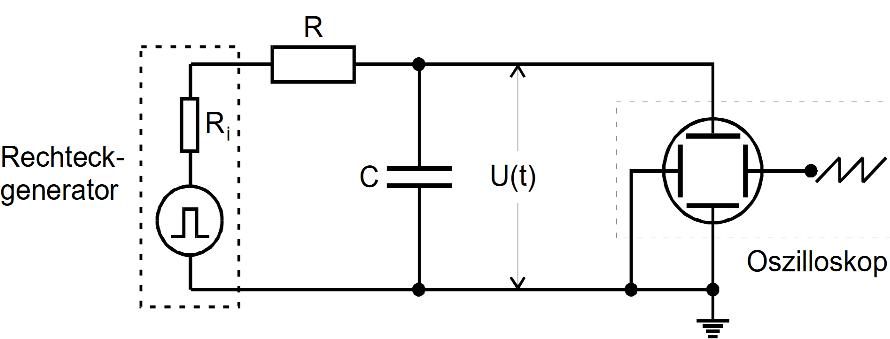
\includegraphics[scale=0.5]{content/images/a.jpg}
\caption{Schaltung zur Bestimmung der Zeitkonstante des RC-Gliedes.\cite{V353}}
\label{fig:a}
\end{figure}
\newline Auf dem Oszilloskop wird ein Entladevorgang des Kondensators betrachtet und zu verschiedenen Zeiten die Spannung gemessen.
\subsection{Amplitude der Kondensatorspannung}
Die Schaltung aus Abbildung \ref{fig:a} bleibt erhalten, wobei der Funktionsgenerator auf Sinusspannung eingestellt wird.
Es wird Frequenz der Generatorspannung variiert und die Amplitude $A$ der Kondensatorspannung für verschiedene Frequenzen gemessen.
Zur Überprüfung der Frequenzunabhängigkeit der Generatorspannung wird das Ozilloskop direkt an das Oszilloskop angeschlossen.
\subsection{Phasenverschiebung zwischen Kondensator- und Generatorspannung}
Es wird eine Schaltung gemäß \ref{fig:c}
aufgebaut. Ein Funktionsgenerator übernimmt dabei die Aufgabe des Frequenzmessers und Sinusgenerators.
\begin{figure}
\centering
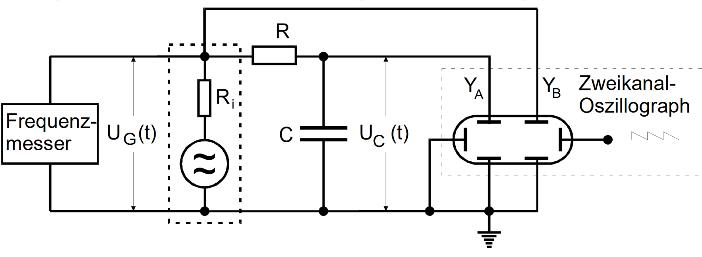
\includegraphics[scale=0.6]{content/images/c.jpg}
\caption{Schaltung zur Bestimmung der Phasendifferenz zwischen Kondensator- und Generatorspannung.\cite{V353}}
\label{fig:c}
\end{figure}
\newline Es wird der Abstand $a$ zwischen den Maxima der beiden auf dem Oszilloskop zu sehenden Spannungen für verschiedene Frequenzen gemessen.
\subsection{Integratoreigenschaft des RC-Gliedes}
Die Schaltung aus Abbildung \ref{fig:c} bleibt erhalten.
Die Generatorspannung wird nacheinander auf eine Sinus-, eine Dreieck- und eine Rechteckspannung gestellt und die resultierenden Spannungsverläufe gespeichert.